%%%%%%%%%%%%%%%%%%%%%%%%%%%%%%%%%%%%%%%%%%%%%%%%%%%%%%%%%%%%%%%%%%%%%%%%%%%%%%%%%%%%%%%%%%%
\section{Discussion}\label{sec:discussion}

\subsection{Solution}

The solution to the differential equation \eqref{eq:susyConditionTheta} is:
\begin{equation}\label{eq:susyConditionSolution}
\boxed{\sin\theta(c) = L \sqrt{c^2-1}; \quad 1 < c \leq \sqrt{1+L^{-2}}, \quad L < 1},
\end{equation}
where $L$ is an integration constant, which is proportional to the mass of the fundamental matter (or quark) field in the dual field theory, as we explain next. The upper bound of $c$ is set by the maximum of the sine.

In the near-boundary limit, $c \approx 1 + z^2/2$, our solution reduces to the exact solution found in the $AdS_5 \times S^5$ background, see \cite{Karch:2002sh} and \cite{Karch:2005ms}, i.e.
\begin{equation}
 \sin\theta(z) = L z.
\end{equation}
As \cite{Karch:2005ms} explains, in the flat embedding space limit, this embedding describes a planar D-brane located at a constant distance $L$ away from the stack of $N$ D3-branes:
\begin{equation}
 L = \lim_{z \rightarrow 0 } \frac{1}{z} \sin\theta(z),
\end{equation}
and this distance is proportional to the quark mass $m$:
\begin{equation}
 L = \dfrac{m}{2 \pi l_s^2}.
\end{equation}


Figures in \ref{fig:vielbeins} show the vielbeins of the induced metric at the solution, from which we learn how the geometry of the embedding looks like at different values of $c$. First, observe the divergence at the horizon $c_{max}=\sqrt{1+M^{-2}}$. This is the location of the well-known enhançon locus, at $\theta = \pi/2$, see \cite{Buchel:2000cn} and \cite{Evans:2000ct}. The spheroid is undeformed at the boundary $c=1$, and becomes squashed until it vanishes at the enhançon. 

\begin{figure}[t!]
\begin{center}
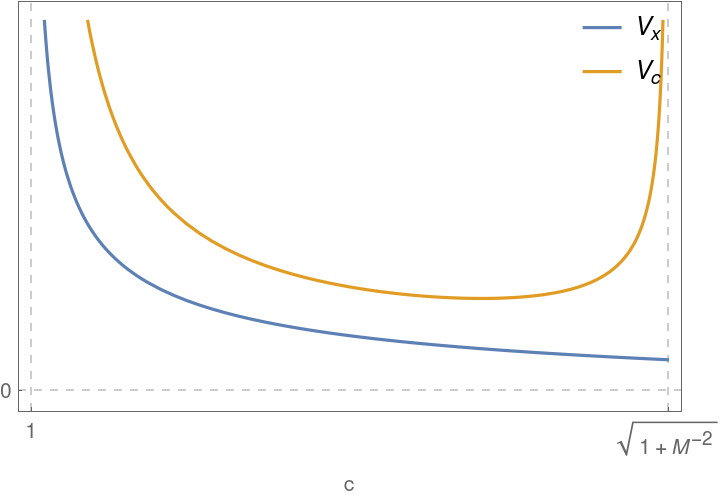
\includegraphics[width=0.6\textwidth]{pictures/vxvc.png}
\end{center}
\vspace{0.05mm}
\begin{center}
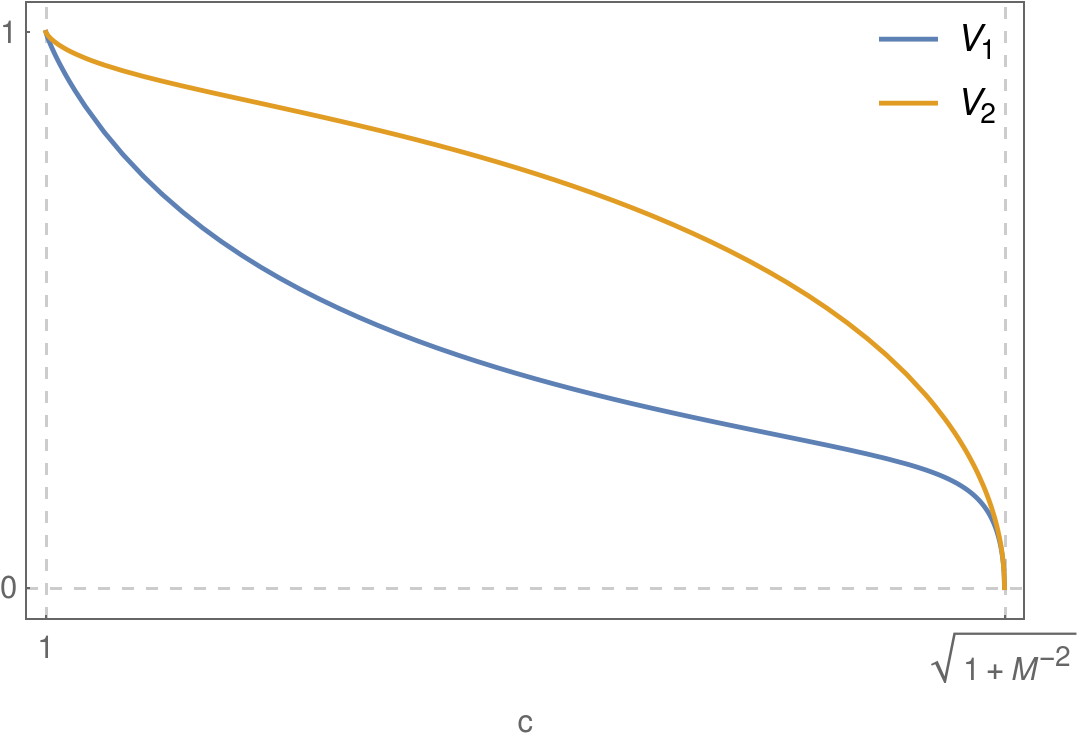
\includegraphics[width=0.6\textwidth]{pictures/v1v2.png}
\end{center}
\caption{\label{fig:vielbeins} The vielbeins of the induced metric at different values of $c$.}
\end{figure}



%%%%%%%%%%%%%%%%%%%%%%%%%%%%%%%%%%%%%%%%%%%%%%%%%%%%%%%%%%%%%%%%%%%%%%%%%%%%%%%%%%%%%%%%%%%%%%%%%
\subsection{Action}


The D7-brane action \eqref{eq:DbraneAction} for our configuration \eqref{eq:ansatz} can be written as:
\begin{align}
 S  = & -T_7 \int_\mathcal{M} d^8\xi \, e^{-P[\Phi] } v_x^4 v_c v_1 v_2^2 \sqrt{1+\frac{v_\theta^2}{v_c^2}\theta'(c)^2}  \nonumber \\
      & + T_7\int _\mathcal{M} P[C_{(8)}],
\end{align}
or more explicitly, using the solution \eqref{eq:susyConditionTheta}, as:
\begin{align}\label{eq:ActionWithTheta'}
 S = & -T_7 \int_\mathcal{M} d^8\xi \, \dfrac{c A(c) \cos^3\theta (c) \sqrt{X_1(c, \theta(c))}}{\left(c^2-1\right)^3} \sqrt{1+ c A(c) \tan^2\theta(c)} \nonumber \\
     & +T_7\int _\mathcal{M} d^8\xi \, \dfrac{A(c)^2 \cos^4\theta(c)}{4 \left(c^2-1\right)^2}.
\end{align}
The explicit form of the Wess-Zumino term is calculated below.

\subsubsection{Wess-Zumino term}
The $P[C_{(8)}]$ term was deemed vanishing in \cite{Albash:2011nw} and \cite{Evans:2005ti}. Their argument did not consider the dilaton factor in the string frame that affects the Hodge star operation while deriving $C_{(8)}$, which in our scenario is
\begin{equation}
 dC_{(8)} = \ast dC_{(0)}.
\end{equation}
The dilaton term from the string frame effectively cancels the factor that vanishes at $\phi_0$, leading to a finite value for the pullback of this potential. We decided to compute it explicitly, and the full result is given in the appendix \ref{sec:backgroundFields}. We can quickly see that it is non-zero for our ansatz for $\phi$ in \eqref{eq:ansatz}. However, $P[C_{(8)}]$ term can be much simpler, as we will see now. First, we can show that:
\begin{equation}\label{eq:C8id}
 [d C_{(8)}]_{\phi_0} = d [C_{(8)}]_{\phi_0}.
\end{equation}
The left-hand-side is simply
\begin{equation}
 [d C_{(8)}]_{\phi_0}  = \dfrac{A^2 \sin\theta \cos^3(\theta)}{\left(c^2-1\right)^2} 
\sigma_1 \wedge \sigma_2 \wedge \sigma_3 \wedge dc  \wedge dx_0 \wedge dx_1 \wedge dx_2 \wedge dx_3 \wedge d\theta,
\end{equation}
and, via \eqref{eq:C8id}, we can integrate the above expression over $\theta$ and obtain:
\begin{equation}
[C_{(8)}]_{\phi_0} = \dfrac{A^2 \cos^4\theta}{4 \left(c^2-1\right)^2} \sigma_1 \wedge \sigma_2 \wedge \sigma_3 \wedge dc \wedge dx_0 \wedge dx_1 \wedge dx_2 \wedge dx_3.
\end{equation}
The full pullback is obtained by just replacing $\theta$ by $\theta(c)$.




%%%%%%%%%%%%%%%%%%%%%%%%%%%%%%%%%%%%%%%%%%%%%%%%%%%%%%%%%%%%%%%%%%%%%%%%%%%%%%%%%%%%%%%%%%%%%%%%%

\subsection{Equation of motion}

As a consistency check for our results, the equation of motion from the action \eqref{eq:ActionWithTheta'} is fulfilled with the solution \eqref{eq:susyConditionTheta}. In particular, 
\begin{align}\label{eq:eom}
-\left.EL[\mathcal{L}_{DBI}]\right|_\text{solution} = EL[\mathcal{L}_{WZ}] = \dfrac{A^2 \sin\theta \cos^3(\theta)}{\left(c^2-1\right)^2},
\end{align}
where $EL[\cdot]$ is the Euler-Lagrange operator:
\begin{equation}
 EL[\mathcal{L}] = 
 \left(\dfrac{\pd }{\pd \theta(c)} -\dfrac{\pd }{\pd c}  \dfrac{\pd }{\pd \theta'(c)} \right) \mathcal{L}.
\end{equation}
Therefore, \eqref{eq:eom} is another proof for the non-vanishing WZ term.



\subsection{Holographic renormalization}
In this subsection, we are going to derive the renormalized action and check that the chiral condensate is zero, as we expect from a supersymmetry embedding.

The fully explicit on-shell action evaluated at the solution \eqref{eq:susyConditionSolution} is:
\begin{align}\label{eq:ActionAtSolution}
 S = & -T_7 \int_\mathcal{M} d^8\xi \, 
 \frac{c A \left(\left(c^2-1\right) L^2-1\right) \left(c \left(c^2-1\right) L^2 A-\left(c^2-1\right) L^2+1\right)}{\left(c^2-1\right)^3}
 \nonumber \\
     & +T_7\int _\mathcal{M} d^8\xi \, 
 \frac{A^2 \left(\left(c^2-1\right) L^2-1\right)^2}{4 \left(c^2-1\right)^2},
\end{align}
where the integration of $c$ is the range shown in \eqref{eq:susyConditionSolution}.

The action is clearly divergent near the boundary, since the geometry of our embedding is asymptotically AdS. Near the boundary, $c \approx 1 + \epsilon^2/2$, with $\epsilon$ small, the divergent terms are:
\begin{align}
 S_\text{div} = T_7 \int_\mathcal{M} d^7\xi 
        \left( \frac{1}{4 \epsilon ^4} +\frac{1-L^2+\log \left(\epsilon/2\right)}{2 \epsilon ^2}-\frac{ \log ^2\left(\epsilon/2\right)}{4}+\frac{\log (\epsilon )}{8} \right).
\end{align}
Both $\log(\epsilon/2)$ terms come from the asymptotic expansion of $A$, which is:
\begin{equation}
 A \approx 1 +\frac{1}{2} \epsilon^2 (2 \log (\epsilon/2)+1) + \frac{1}{8} \epsilon^4 (2 \log(\epsilon/2)-1) + \ldots
\end{equation}


Let us renormalize the action using the holographic renormalization \cite{Bianchi:2001kw}. Essentially, it amounts in cancelling the divergences of the on-shell action by adding covariant local counterterms determined by the near-boundary behavior of bulk fields. That said, the renormalized action in the form of \eqref{eq:ActionWithTheta'} with the counterterms is
\begin{align}\label{eq:ActionWithTheta'}
 S_\text{ren} = & -T_7 \int_\mathcal{M} d^8\xi \, \dfrac{c A(c) \cos^3\theta (c) \sqrt{X_1(c, \theta(c))}}{\left(c^2-1\right)^3} \nonumber\\
               &\left(\sqrt{1+ c A(c) \tan^2\theta(c)} - 1 - \frac{1}{2} c A(c) \theta (c)^2 - \frac{5}{24}\theta (c)^4 \right) \nonumber \\
     & +T_7\int _\mathcal{M} d^8\xi \, \dfrac{A(c)^2}{4 \left(c^2-1\right)^2}\left(\cos^4\theta(c) - 1 + 2 \theta(c)^2\right).
\end{align}
The counterterms for the DBI part are essentially the counterterms $L_1$, $L_4$ and $L_f$ derived in section 4 of \cite{Karch:2005ms}. From the same reference, the chiral condensate is sourced by the leading order coefficient of the near-boundary expansion of the scalar field, which in our case is:
\begin{equation}
 \theta(\epsilon) \approx L \, \epsilon + \ldots,
\end{equation}
thus
\begin{equation}
\langle O \rangle = \frac{1}{\sqrt{g_{(0)}}} \frac{\delta S_\text{ren}}{\delta L} \right),
\end{equation}
where $g_{(0)}$ is the leading finite part of the metric, see definition in \cite{Karch:2005ms}.



The condensate is indeed zero. We can see that the action is proportional to $\theta(\epsilon)^4$ near the boundary. Therefore, the functional derivative is proportional to $L^3 \epsilon^4$, which vanishes when we remove the regulator $\epsilon \rightarrow 0$.



 




